\documentclass[tikz,border=8pt]{standalone}
\usepackage{tikz}
\usetikzlibrary{arrows.meta,positioning,fit,backgrounds}

\definecolor{kmblue}{RGB}{0,56,116}
\definecolor{kmgold}{RGB}{160,120,0}
\definecolor{rtgreen}{RGB}{30,130,60}
\definecolor{rscol}{RGB}{100,80,160}
\definecolor{sharedcol}{RGB}{0,130,120}
\definecolor{apcol}{RGB}{150,30,30}
\definecolor{lightblue}{RGB}{220,235,255}
\definecolor{lightgreen}{RGB}{210,240,220}
\definecolor{lightpurple}{RGB}{235,225,255}
\definecolor{lightcyan}{RGB}{210,245,245}

\begin{document}
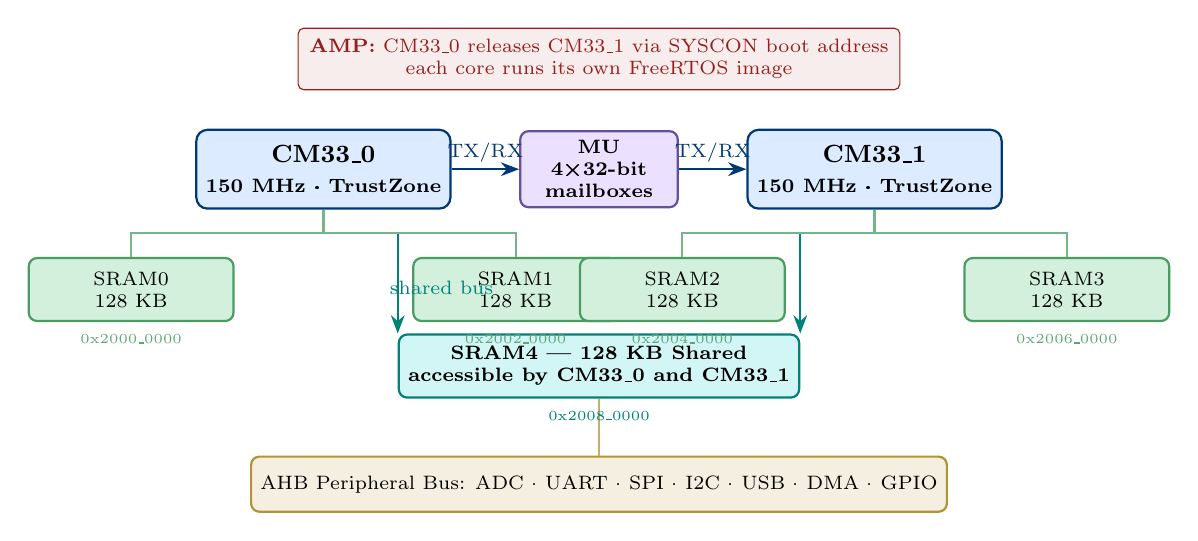
\begin{tikzpicture}[
  core/.style={draw=kmblue, fill=lightblue, thick, rounded corners=4pt,
               minimum width=3.2cm, minimum height=1.0cm,
               font=\small\bfseries, align=center},
  sram/.style={draw=rtgreen!80, fill=lightgreen, thick, rounded corners=3pt,
               minimum width=2.6cm, minimum height=0.8cm,
               font=\scriptsize, align=center},
  shared/.style={draw=sharedcol, fill=lightcyan, thick, rounded corners=3pt,
                 minimum width=3.0cm, minimum height=0.8cm,
                 font=\scriptsize\bfseries, align=center},
  mu/.style={draw=rscol, fill=lightpurple, thick, rounded corners=3pt,
             minimum width=2.0cm, minimum height=0.8cm,
             font=\scriptsize\bfseries, align=center},
  periph/.style={draw=kmgold!80, fill=kmgold!12, thick, rounded corners=3pt,
                 minimum width=5.8cm, minimum height=0.7cm,
                 font=\scriptsize, align=center},
  lbl/.style={font=\scriptsize, inner sep=2pt},
  arrow/.style={->, >=Stealth, thick},
]

% ---- CM33_0 ----
\node[core] (cm0) at (0,0) {CM33\_0\\{\scriptsize 150 MHz · TrustZone}};

% CM33_0 private SRAMs
\node[sram, below left=0.6cm and -0.5cm of cm0] (s0) {SRAM0\\128 KB};
\node[sram, below right=0.6cm and -0.5cm of cm0] (s1) {SRAM1\\128 KB};

% ---- CM33_1 ----
\node[core] (cm1) at (7,0) {CM33\_1\\{\scriptsize 150 MHz · TrustZone}};

% CM33_1 private SRAMs
\node[sram, below left=0.6cm and -0.5cm of cm1] (s2) {SRAM2\\128 KB};
\node[sram, below right=0.6cm and -0.5cm of cm1] (s3) {SRAM3\\128 KB};

% ---- Messaging Unit ----
\node[mu] (mu) at (3.5,0) {MU\\4×32-bit\\mailboxes};

% ---- Shared SRAM4 ----
\node[shared] (s4) at (3.5,-2.5) {SRAM4 — 128 KB Shared\\accessible by CM33\_0 and CM33\_1};

% ---- Peripherals bar ----
\node[periph] (periph) at (3.5,-4.0)
  {AHB Peripheral Bus: ADC · UART · SPI · I2C · USB · DMA · GPIO};

% ---- Connections ----
% MU <-> cores
\draw[arrow, kmblue] (cm0.east) -- (mu.west)
  node[midway,above,lbl]{TX/RX};
\draw[arrow, kmblue] (mu.east) -- (cm1.west)
  node[midway,above,lbl]{TX/RX};

% SRAM4 <-> both cores (data bus)
\draw[arrow, sharedcol] (cm0.south) -- ++(0,-0.3) -| (s4.north west)
  node[near end,left,lbl,sharedcol]{};
\draw[arrow, sharedcol] (cm1.south) -- ++(0,-0.3) -| (s4.north east);
\node[lbl, sharedcol] at (1.5,-1.5){\scriptsize shared bus};

% Private SRAMs
\draw[rtgreen!60, thick] (cm0.south) -- ++(0,-0.3) -| (s0.north);
\draw[rtgreen!60, thick] (cm0.south) -- ++(0,-0.3) -| (s1.north);
\draw[rtgreen!60, thick] (cm1.south) -- ++(0,-0.3) -| (s2.north);
\draw[rtgreen!60, thick] (cm1.south) -- ++(0,-0.3) -| (s3.north);

% Peripherals
\draw[kmgold!60, thick] (s4.south) -- (periph.north);

% ---- AMP label ----
\node[draw=apcol, rounded corners=2pt, fill=apcol!8,
      font=\scriptsize, align=center, inner sep=4pt,
      text=apcol]
     (amp) at (3.5,1.4)
  {\textbf{AMP:} CM33\_0 releases CM33\_1 via SYSCON boot address\\
   each core runs its own FreeRTOS image};

% ---- Addresses ----
\node[font=\tiny, rtgreen!70, below=1pt of s0]{0x2000\_0000};
\node[font=\tiny, rtgreen!70, below=1pt of s1]{0x2002\_0000};
\node[font=\tiny, rtgreen!70, below=1pt of s2]{0x2004\_0000};
\node[font=\tiny, rtgreen!70, below=1pt of s3]{0x2006\_0000};
\node[font=\tiny, sharedcol, below=1pt of s4]{0x2008\_0000};

\end{tikzpicture}
\end{document}
